%% AQB, Apart Research hackathon submission format (<= 8 pages).
%% Build: pdflatex main && bibtex main && pdflatex main && pdflatex main
\documentclass[10pt,letterpaper]{article}
\usepackage[margin=0.9in,top=0.8in,bottom=0.8in]{geometry}
\usepackage[T1]{fontenc}
\usepackage{librebaskerville}
\usepackage{microtype}
\usepackage{amsmath}
\usepackage{graphicx}
\usepackage{booktabs}
\usepackage{enumitem}
\usepackage[numbers,sort&compress]{natbib}
\usepackage[colorlinks=true,linkcolor=black,citecolor=black,urlcolor=blue!50!black]{hyperref}
\usepackage{xcolor}
\usepackage{titlesec}
\usepackage{xspace}
\usepackage{tikz}
\usetikzlibrary{positioning,arrows.meta,fit,calc}
\usepackage{caption}
\captionsetup{font=small,labelfont=bf,skip=3pt}
\setlist{nosep,leftmargin=*}
\setlength{\parskip}{3pt}
\setlength{\parindent}{0pt}
\setlength{\bibsep}{0pt}
\titleformat{\section}{\large\bfseries}{\thesection.}{0.5em}{}
\titleformat{\subsection}{\bfseries}{}{0pt}{}
\titleformat{\paragraph}[runin]{\bfseries}{}{0pt}{}[.]
\titlespacing*{\section}{0pt}{9pt}{3pt}
\titlespacing*{\subsection}{0pt}{6pt}{2pt}
\titlespacing*{\paragraph}{0pt}{4pt}{6pt}
\newcommand{\aqb}{AQB\xspace}
\newcommand{\answer}[2]{\par\noindent\textit{Answer to RQ#1.} #2}
\renewcommand{\thefootnote}{\arabic{footnote}}

\begin{document}

\noindent\rule{\textwidth}{2.2pt}\par\vspace{10pt}
\begin{center}
{\LARGE\bfseries CAN LLM AGENTS HOLD THE RELEASE GATE?\textsuperscript{1}}\\[4pt]
{\large\bfseries A Benchmark of Device-Verified Regressions in Real Android Apps}
\end{center}
\vspace{2pt}\noindent\rule{\textwidth}{0.5pt}\par\vspace{8pt}
\begin{center}
Mayank Singh\\ Independent researcher\\[5pt]
{\bfseries With}\\Apart Research
\end{center}
\vspace{2pt}
\begin{center}{\large\bfseries Abstract}\end{center}\vspace{-4pt}
\begin{quote}\itshape\small
Coding agents produce changes faster than people can test them, so the release gate, a human tester
who exercises what changed and either files bugs or signs off, is becoming the bottleneck. We ask
whether an LLM agent can hold that gate and whether its reports and sign-offs can be trusted. We
present \aqb, 51 release-QA episodes over 9 open-source Android apps. Each episode is a build with one
to three planted regressions (92 in total, 91 observable), each a real upstream bug re-introduced on a
pinned head commit and verified on a device. The agent gets release notes that name every changed
feature without a symptom, drives an Android~15 device through screen tools, files bug reports, and
decides when to sign off. A deterministic matcher grades reports without a model judge. Across six
configurations from three providers, the best recall is 59.3\% and the best strict pass rate (every
regression reported, then a sign-off) is 29.4\%; 17 of 91 regressions escape every configuration.
Agents reach 74--96\% of the changed features but rarely run the checks that expose the regressions:
reopening after a change, specific inputs, and comparing a value with what it should be. The
confidence an agent states with its sign-off is close to chance at separating correct from incorrect
sign-offs (AUROC 0.33--0.58).
\end{quote}
\footnotetext[1]{Research conducted at the \href{https://apartresearch.com}{AI x Epistemics Research Sprint}, November 2026.}

%% ---------------------------------------------------------------------------------
\section{Introduction}
A team that uses coding agents can produce changes faster than people can test them. The last check
before release is often still a tester who reads the release notes, exercises what changed, and
either files bugs or signs off. That person is the \emph{test oracle}, the judge of whether observed
behaviour is correct, and when no automated oracle is adequate the human remains the final source of
that information~\cite{barr2015oracle}. The task combines regression testing~\cite{yoo2012regression}
with exploratory testing~\cite{itkonen2005exploratory}. If agents take this role, the failure that
matters for safety is not a missed demo but a confident sign-off on a build that still contains a
regression.

Existing benchmarks measure other things. Software-engineering benchmarks grade code an agent
writes~\cite{jimenez2024swebench,merrill2026terminalbench}; Android and computer-use benchmarks grade
task completion in apps assumed to be correct~\cite{rawles2025androidworld,xu2025androidlab,xie2024osworld};
GUI-testing research measures test generators on coverage and crashes~\cite{li2017droidbot,mao2016sapienz,su2017stoat,su2021themis}.
No existing benchmark asks an LLM agent to act as a release gate: sweep a build from its
release notes, report what is wrong, and decide when it can ship.

\textbf{Our main contributions are:}
\begin{enumerate}
\item \aqb, a benchmark of 92 planted, device-verified regressions (91 observable) in 9 real Android
  apps, organised into 51 release-QA episodes with 92 real and 93 decoy release-note lines.
\item A deterministic, model-free matcher for free-text bug reports, anchored to what was on screen,
  checked on a corpus of reports written without the keys.
\item An evaluation of six agent configurations from three providers in their vendors' own harnesses,
  with intervals, corrected pairwise tests and sensitivity analyses.
\item A per-feature account of every miss (never reached, reached but not exercised, exercised but not
  noticed), the regressions that all strong configurations miss.
\end{enumerate}

\begin{figure}[t]
  \centering
  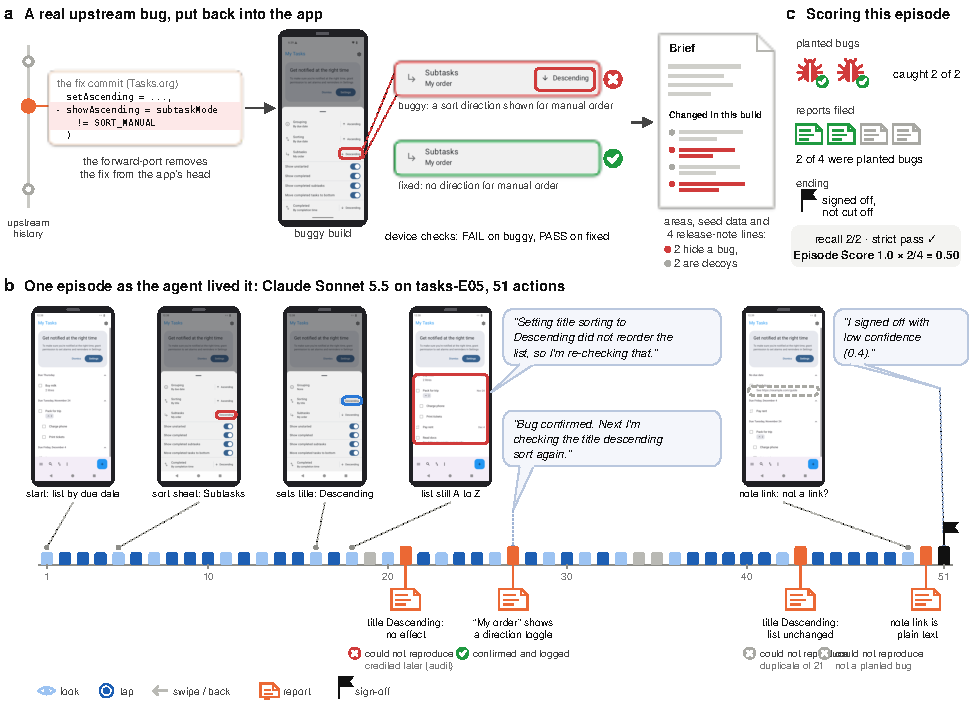
\includegraphics[width=0.93\textwidth]{../figures/p0_overview.pdf}
  \caption{\aqb at a glance, with real artifacts from one episode. \textbf{a}, A regression enters a
  build: the fix of an upstream Tasks.org bug is reversed on the pinned head; the buggy build shows a
  sort-direction toggle for a manually ordered list that the fixed build does not. \textbf{b}, The same
  episode as executed by Claude Sonnet~5.5: screenshots, its words, its 51 actions, four reports with
  the scripted developer's replies, and the sign-off. \textbf{c}, How the episode is scored.}
  \label{fig:overview}
\end{figure}

%% ---------------------------------------------------------------------------------
\section{Related Work}
\paragraph{Agent benchmarks for software and mobile}
SWE-bench grades patches against repository tests~\cite{jimenez2024swebench}; Terminal-Bench grades
shell tasks~\cite{merrill2026terminalbench}. AndroidWorld, AndroidLab and OSWorld use programmatic
success checks in apps assumed correct~\cite{rawles2025androidworld,xu2025androidlab,xie2024osworld}.
In \aqb the app contains defects the agent must discover, and success depends on its judgement of
whether what it sees is correct.
\paragraph{Android GUI testing}
Random, search-based and model-based generators~\cite{li2017droidbot,mao2016sapienz,su2017stoat} are
evaluated on coverage and crashes; Themis uses real crash bugs~\cite{su2021themis}. Non-crashing
functional bugs are targeted with derived or generic oracles~\cite{su2021genie,wang2022deepstate,liu2025guipilot},
and LLM testers such as GPTDroid, DroidAgent and VisionDroid report bugs found~\cite{liu2024gptdroid,yoon2024droidagent,liu2025visiondroid}.
These works propose tools; \aqb measures the release-gate decision itself, with release notes as the
only guide and a sign-off that ends the session. Like Defects4J~\cite{just2014defects4j}, each bug
comes from a real upstream fix, but it is observed only through the screen.

%% ---------------------------------------------------------------------------------
\section{Methods}
\paragraph{Apps and regressions}
\aqb uses 9 open-source apps (Amaze File Manager, AnkiDroid, Markor, Tasks.org, Minus, Iris Gallery,
Featherline, NerdCalci, Idle Fantasy); four are mature projects and five have history only from 2026.
Each is pinned to one head commit. A regression starts from a merged upstream fix whose bug (i) shows
on screen or in displayed data, (ii) is deterministic, and (iii) can be judged wrong without the code.
At least 256 fixes were examined, 163 were authored and forward-ported, and 101 were verified on a
device; 92 are planted in episodes. Regressions are labelled state (38), display (35) or interaction
(19). The buggy build is the head plus a patch reversing the fix; the fixed build is the clean head.
Each bug has three deterministic device checks: a \emph{target} check of its trigger, a
\emph{held-out} check reaching the defect by another path, and a \emph{preservation} check of
neighbouring behaviour. A bug is accepted only if target and held-out fail on the buggy build and pass
on the fixed one, and preservation passes on both.

\begin{table}[t]
  \centering
  \caption{Apps and planted regressions. Amaze's count includes one regression another bug in its
  episode masks; 91 are observable.}
  \label{tab:apps}
  \small\setlength{\tabcolsep}{6pt}
  \begin{tabular}{@{}llllrr@{}}
    \toprule
    App & Domain & Licence & History & Episodes & Regressions \\
    \midrule
    Amaze File Manager & file manager & GPL-3.0 & mature & 6 & 12 (11) \\
    AnkiDroid & flashcards & GPL-3.0 & mature & 8 & 15 \\
    Markor & Markdown editor & Apache-2.0 & mature & 6 & 13 \\
    Tasks.org & to-do lists & GPL-3.0 & mature & 6 & 12 \\
    Minus & expense tracker & Apache-2.0 & 2026 & 6 & 8 \\
    Iris Gallery & photo gallery & Apache-2.0 & 2026 & 3 & 3 \\
    Featherline & medication tracker & GPL-3.0 & 2026 & 6 & 9 \\
    NerdCalci & notepad calculator & GPL-3.0 & 2026 & 4 & 8 \\
    Idle Fantasy & idle RPG & GPL-3.0 & 2026 & 6 & 12 \\
    \midrule
    Total & & & & 51 & 92 (91) \\
    \bottomrule
  \end{tabular}
\end{table}

\paragraph{Episodes and release notes}
An episode groups one to three regressions of one app that touch different files (16, 29 and 6
episodes with one, two and three). The brief names the areas to sweep, the seeded data and a
\emph{Changed in this build} list with one line per regression plus one or two harmless decoys. Lines
name the feature and what changed in its mechanism, never a symptom, trigger or expected value, and
real and decoy lines use the same verbs. A leak scan checks briefs for bug identifiers and
fix-commit wording.

\paragraph{Environment}
Each episode runs on a fresh Android~15 container. The agent reaches it only through a Model Context
Protocol server~\cite{anthropic2024mcp} (\texttt{observe}, \texttt{tap}, \texttt{type\_text},
\texttt{swipe}, \texttt{rotate}, \texttt{open\_app}, \ldots) plus \texttt{file\_report} and
\texttt{sign\_off}; its harness has all other tools disabled and runs in an empty directory. The
prompt contains the brief, a short generic QA method (plan every area, check state after leaving and
returning, reverse and repeat actions, try empty and boundary inputs, rotate, reach screens by more
than one route) and finishing instructions. A report gives a screen, element, symptom type, expected
and observed behaviour, steps, and where possible the exact on-screen quote showing the defect. A
scripted developer answers ``confirmed'', ``already logged'' or ``cannot reproduce''. An episode ends
at sign-off, when the agent stops, at 300 actions (undisclosed), or after $2n{+}3$ reports for $n$
planted bugs.

\begin{figure}[t]
  \centering
  \begin{tikzpicture}[
      blk/.style={draw, rounded corners=2pt, align=center, font=\scriptsize, minimum height=9mm, fill=white},
      grp/.style={draw, dashed, rounded corners=3pt, inner sep=4pt},
      arr/.style={-{Latex[length=1.6mm]}, semithick},
      lab/.style={font=\scriptsize\itshape, align=center}]
    \node[blk, text width=2.9cm] (agent) {LLM agent in its vendor harness\\(Claude Code, Codex CLI,\\DeepSeek Harness)};
    \node[blk, text width=2.9cm, right=9mm of agent] (mcp) {MCP device server\\observe, tap, type, swipe,\\rotate, \ldots};
    \node[blk, text width=3.0cm, right=9mm of mcp] (ctrl) {Evaluation controller\\action cap 300, report\\limit $2n{+}3$, transcript};
    \node[blk, text width=2.6cm, right=9mm of ctrl] (dev) {Android 15 container\\start build + seed data};
    \node[blk, text width=3.0cm, below=8mm of ctrl] (rep) {\texttt{file\_report} $\rightarrow$\\deterministic matcher};
    \node[blk, text width=3.4cm, left=9mm of rep] (dvp) {Scripted developer: ``confirmed'' / ``already logged'' / ``cannot reproduce''};
    \node[blk, text width=2.6cm, right=9mm of rep] (so) {\texttt{sign\_off}\\(ends the session)};
    \node[grp, fit=(agent), label={[lab]above:no shell, files or web;\\empty working directory}] {};
    \draw[arr] (agent) -- (mcp);
    \draw[arr] (mcp) -- (ctrl);
    \draw[arr] (ctrl) -- node[lab, above]{adb} (dev);
    \draw[arr] (ctrl) -- (rep);
    \draw[arr] (rep) -- (dvp);
    \draw[arr] (ctrl) -- (so);
    \draw[arr] (dvp.west) -| (agent.south);
  \end{tikzpicture}
  \caption{Episode environment. The agent reaches the device only through the MCP server; every call
  is executed and logged by the controller. Reports are graded online and answered by a scripted
  developer; a confirmed regression stays in the build.}
  \label{fig:arch}
\end{figure}

\paragraph{Deterministic grading}
LLM judges show position, verbosity and self-enhancement bias~\cite{zheng2023judge}, and a judge from
one provider grading agents from several favours its own family, so we use hand-written keys and
accept a measured recall ceiling. A report is credited to a planted regression when (1) its screen,
element or field matches the key's location concepts or anchor element, (2) its expected and observed
text match every concept group of the intended behaviour and the defect (numbers as whole numbers
only), and (3) its quote, when usable, was on screen in that session. Mirrored, vague, multi-defect
or overlong reports are rejected first; a report credits at most one regression, uncredited first.
On a corpus of 606 reports written without the keys, the matcher credits 84.2\% of correct reports and
never credits the wrong regression within an episode.

\paragraph{Metrics}
For episode $e$ let $B_e$ be its observable regressions, $C_e\subseteq B_e$ the credited ones, $F_e$
the false reports, $s_e$ whether the agent signed off, and $k_e$ whether the controller cut it off.
\emph{Recall} is $\sum|C_e|/\sum|B_e|$. \emph{Strict pass} is the share of episodes with $C_e=B_e$ and
a sign-off, the release-gate view. The \emph{Episode Score} averages
$\mathrm{cc}(|C_e|,|B_e|)\cdot\pi_e\cdot(\tfrac12)^{k_e}$, where $\mathrm{cc}(c,b)=\frac{1+(c-1)/2}{1+(b-1)/2}$
($0$ for $c=0$) is a diminishing catch credit and $\pi_e=|C_e|/(|C_e|+F_e)$ the report precision.
\emph{Changelog coverage} classifies each release-note line from the transcript alone as reached (a
UI string appeared), exercised (six or more actions with the feature on screen) and caught; a miss is
\emph{ignored}, \emph{shallow} or \emph{not noticed}. Intervals are 95\% bootstrap CIs resampling whole
episodes~\cite{efron1979} (Wilson for strict pass~\cite{wilson1927}); pairwise tests are paired
sign-flip permutation tests over the 51 episodes with Holm correction~\cite{holm1979}; catch overlap
is tested by a hypergeometric tail; confidence is summarised by AUROC~\cite{hanley1982auc}.

\paragraph{Configurations}
Each model runs in its vendor's harness at its default effort, and GPT-6 Luna also at maximum: Claude
Sonnet~5.5 and Claude Haiku~5.5 (Claude Code), GPT-6.1 Sol and GPT-6 Luna at medium and max (Codex
CLI), and DeepSeek V4.1 Flash (DeepSeek Harness). No configuration gets more actions, time or reports
than another. Each ran all 51 episodes once. Sonnet, Haiku and DeepSeek used episode prompt v4; Sol and
Luna used v4.1, which tightens the wording of the sign-off instruction (Section~\ref{sec:threats}).

%% ---------------------------------------------------------------------------------
\section{Results}
We ask \textbf{RQ1} how well agents hold the gate, \textbf{RQ2} whether their reports and sign-offs can be
trusted, \textbf{RQ3} how effort and cost relate to score, and \textbf{RQ4} where and why they miss.

\begin{table}[t]
  \centering
  \caption{Main results on 51 episodes (one run each). Recall and Episode Score: 95\% bootstrap CI;
  strict pass: Wilson CI. Cost: mean per episode at API list prices ($^\ast$mean over 50 sessions).}
  \label{tab:main}
  \small\setlength{\tabcolsep}{4pt}
  \begin{tabular}{@{}lrrrrrr@{}}
    \toprule
    Configuration & Recall (\%) & Strict pass (\%) & Prec. (\%) & Episode Score & Actions & \$/ep. \\
    \midrule
    Sol & \textbf{59.3} [50.0, 68.5] & \textbf{29.4} [18.7, 43.0] & 34.0 & 0.29 [0.22, 0.36] & 202 & 0.65 \\
    DeepSeek & 50.5 [40.0, 60.4] & 11.8 [5.5, 23.4] & 34.1 & 0.18 [0.12, 0.25] & 294 & 0.06 \\
    Sonnet & 46.2 [36.3, 55.7] & 23.5 [14.0, 36.8] & 44.2 & \textbf{0.39} [0.29, 0.50] & 67 & 0.54 \\
    Haiku & 42.9 [31.1, 53.9] & 13.7 [6.8, 25.7] & 27.7 & 0.24 [0.16, 0.32] & 217 & 0.64 \\
    Luna max & 34.1 [23.9, 44.0] & 11.8 [5.5, 23.4] & 24.4 & 0.21 [0.13, 0.29] & 166 & 0.16$^\ast$ \\
    Luna med. & 15.4 [8.6, 23.2] & 3.9 [1.1, 13.2] & \textbf{50.0} & 0.14 [0.07, 0.22] & 39 & 0.02 \\
    \bottomrule
  \end{tabular}
\end{table}

\subsection{RQ1: Holding the gate}
Table~\ref{tab:main} gives the main results. The best recall is 59.3\% (Sol) and the best strict pass
rate 29.4\%: in seven of ten releases even the best configuration ships a regression or ends
without a verdict. Over all six configurations 74 of 91 regressions (81\%) are caught at least once and
17 by none. After Holm correction Sol and DeepSeek beat Luna max on recall, and Sol, DeepSeek, Sonnet
and Haiku beat Luna med.\ ($p_{\text{Holm}}\le0.011$); no difference among the four strongest is
significant. Sol catches 22 regressions Sonnet misses and Sonnet 10 that Sol misses
($p_{\text{Holm}}=0.17$).
\answer{1}{No configuration holds the gate reliably: the best catches 59\% of regressions and strictly
passes 29\% of releases.}

\begin{figure}[t]
  \centering
  \includegraphics[width=\textwidth]{figs/headline.pdf}
  \caption{Headline metrics with 95\% intervals (Table~\ref{tab:main}); colour and marker encode the
  provider, rows are ordered by recall.}
  \label{fig:headline}
\end{figure}

\subsection{RQ2: Trusting reports and sign-offs}
The configuration that finds the most is not the most trustworthy. Sol files 164 reports and 54 are
credited (precision 34\%); Sonnet files 99 and 42 are credited (44\%). With precision counted, Sonnet
has the highest Episode Score (0.39), significantly above DeepSeek, Luna max and Luna med.\
($p_{\text{Holm}}\le0.006$) but not above Haiku or Sol ($+0.10$, $p_{\text{Holm}}=0.66$), so neither
leaderboard position is established.

\begin{figure}[t]
  \centering
  \includegraphics[width=0.49\textwidth]{figs/endings.pdf}\hfill
  \includegraphics[width=0.49\textwidth]{figs/confidence.pdf}
  \caption{\textbf{Left:} how each of the 51 episodes ended. \textbf{Right:} stated sign-off confidence
  for sign-offs after which every regression had been reported (circles) and sign-offs that left
  regressions (crosses), with AUROC per configuration.}
  \label{fig:endings}
\end{figure}

Sonnet and both Luna settings sign off in almost every episode, yet 76--90\% of all their episodes end
in a sign-off with regressions still present (Figure~\ref{fig:endings}, left). DeepSeek is cut off at
the action cap in 78\% of episodes. No configuration signs off correctly in more than 29\%. The
confidence stated with a sign-off does not separate correct from incorrect ones (Figure~\ref{fig:endings},
right): AUROC is 0.53--0.58 for five configurations and 0.33 for Haiku, whose confidence is
inverted. Each configuration instead has a typical value: 0.5 for the Claude models and 0.75--0.9
for the GPT and DeepSeek configurations. This is the miscalibration known from neural networks~\cite{guo2017calibration}.
\answer{2}{No. The highest-recall configuration files two false reports per credited one, most
sign-offs leave regressions in the build, and stated confidence is near chance.}

\subsection{RQ3: Effort and cost}
Across configurations, actions do not predict the Episode Score (Spearman $\rho=0.03$, $n=6$): Sonnet
scores highest with 67 actions per episode while Sol, Haiku and DeepSeek use 200--300 and score lower.
Within one model more effort helps: raising GPT-6 Luna from medium to maximum raises actions from 39
to 166, recall from 15\% to 34\% and score from 0.14 to 0.21, while precision falls from 50\% to 24\%.
Cost and score are positively associated ($\rho=0.83$, $n=6$; six points, no test). The
Artificial Analysis index~\cite{aa2026index} ranks the four configurations with an entry similarly
($\rho=0.80$, $n=4$), except that it places Sol (35) above Sonnet (31) where the Episode Score
reverses them.
\begin{figure}[t]
  \centering
  \includegraphics[width=\textwidth]{figs/effort_cost.pdf}
  \caption{Episode Score against (a) mean agent actions per episode (dashed: the 300-action cap) and
  (b) cost per episode at API list prices (log scale). Hollow marker: cost known for 50 of 51 sessions.}
  \label{fig:effort}
\end{figure}
\answer{3}{More actions across configurations do not mean a higher score; within GPT-6 Luna, more
reasoning effort raised recall and score.}

\subsection{RQ4: Where agents miss}
\begin{figure}[t]
  \centering
  \includegraphics[width=0.49\textwidth]{figs/coverage.pdf}\hfill
  \includegraphics[width=0.49\textwidth]{figs/recall_precision.pdf}
  \caption{\textbf{Left:} what happened to each of the 92 release-note lines hiding a regression
  (caught, exercised but not noticed, reached but not exercised, never reached).
  \textbf{Right:} recall against report precision; dotted lines join equal F1.}
  \label{fig:coverage}
\end{figure}

\paragraph{Agents reach the features but do not expose the regressions}
Every configuration except Luna med.\ reaches 78--88 of the 92 changed features (Figure~\ref{fig:coverage}).
The misses lie in what agents do there: 23--46 regressions per configuration sit in features the agent
exercised with six or more actions without exposing them. Sonnet looks only briefly: 23 of its 42 catches
came from features it looked at for fewer than six actions.

\paragraph{Configurations share a difficulty structure}
Catches overlap more than chance for all 15 pairs (observed-to-expected shared catches 1.28--2.29;
Jaccard 0.22--0.54; $p_{\text{Holm}}\le0.022$). For Sol and Sonnet, 32 shared catches compare with
24.9 expected. 17 regressions are caught by none and 11 by all six, so each regression has a stable difficulty. Splits by app age, fix date and family change the order of the four strongest
configurations by at most one place.

\begin{figure}[t]
  \centering
  \includegraphics[width=\textwidth]{figs/difficulty.pdf}
  \caption{(a) Number of configurations that caught each observable regression. (b) For each pair of
  configurations, shared catches divided by the number expected under independence; every ratio exceeds
  1 ($p_{\text{Holm}}\le0.022$).}
  \label{fig:difficulty}
\end{figure}

\paragraph{The regressions both leading configurations miss}
The 27 regressions that both Sol and Sonnet missed are no older and were not ported with lower
confidence. By what a tester must do, they fall into: \emph{round trip} (6), change a setting, close
and reopen, check the value; \emph{specific input or action} (10), such as long-pressing \emph{Bold}
(which closes the app), choosing \emph{Select all} twice, or typing seven digits into a five-digit
field; \emph{knowing the correct value} (10), where the screen looks plausible, as with 2,567,890
coins shown as 2.6M where the format floors to 2.5M, or a Videos filter that says ``No photos found'' (Figure~\ref{fig:hard});
and \emph{multi-step state} (1). The first two groups map directly onto instructions in the prompt, which
also says that signing off with bugs unreported is the worst outcome. The logs show how rarely those
checks ran: Sonnet re-opened the app in 13 of 51 episodes, and Sol rotated the device in every episode
but long-pressed an element in only 7. Sol and DeepSeek spent 133 and 151 actions on the Markor
formatting toolbar without long-pressing \emph{Bold}.

\begin{figure}[t]
  \centering
  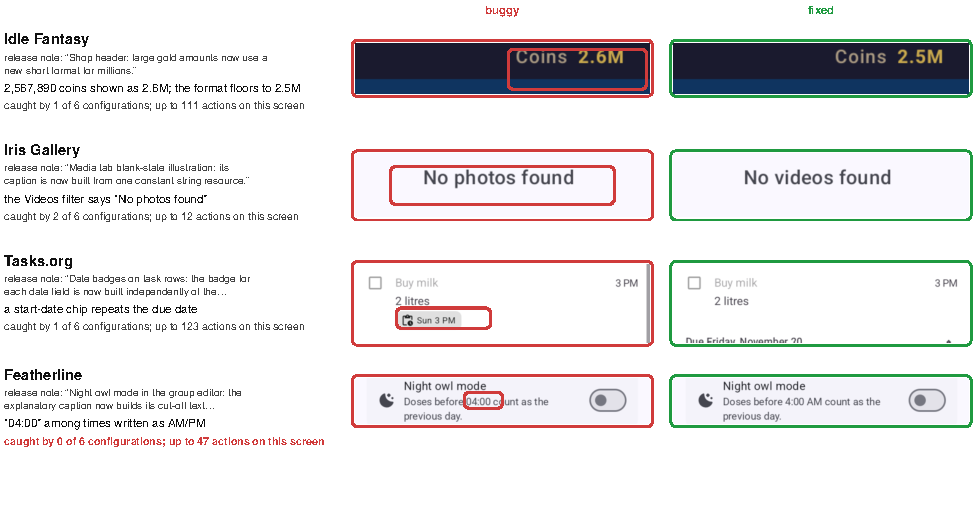
\includegraphics[width=0.85\textwidth]{../figures/p7_hard.pdf}
  \caption{Regressions that both Sol and Sonnet missed, as the device shows them on the buggy and fixed
  builds (defect circled), with the release-note line the agent received.}
  \label{fig:hard}
\end{figure}

\paragraph{Contamination}
Comparing regressions fixed before 2026 (33) with those fixed in 2026 (58), no configuration differs
significantly (Fisher's exact test, all $p\ge0.24$, no consistent sign). This tests the fix date, not
each model's training cut-off, so it cannot rule out contamination~\cite{sainz2023contamination}.
\answer{4}{Agents miss regressions in features they did exercise, because they skip the specific
check that exposes them; hard regressions are hard for every configuration.}

%% ---------------------------------------------------------------------------------
\section{Discussion and Limitations}
\paragraph{Implications for AI safety and oversight}
Delegating release sign-off to an agent is an oversight decision, and these results argue against it at
current performance: a deployment that did so would ship regressions in most releases, and the
confidence the agent reports gives no usable warning. Which metric matters depends on the gate. With a
human reviewing reports, a missed regression is costly and recall ranks the configurations (Sol leads);
if reports go to developers directly, precision and correct sign-off matter and the Episode Score
ranks them (Sonnet leads); for an unattended gate, strict pass is the metric. The misses
concentrate in verification steps agents were told to use, so the remedy is scaffolding that enforces the
method, such as a per-feature checklist of round trips and boundary inputs, not a larger exploration
budget; we have not tested this. The union of all six configurations still misses 19\% of regressions.

\paragraph{Limitations}\label{sec:threats}
\textbf{Internal.} Sonnet, Haiku and DeepSeek ran episode prompt v4; Sol and Luna ran v4.1, which
tightens the sign-off instruction. The weaker models took the v4 wording literally, which v4.1 corrects;
the larger models were not affected by it. Harness and model effects are not separated, and each
configuration ran each episode once, so part of the difference in which regressions are caught is
run-to-run variance. The matcher credits 84\% of correct reports, so recall is a lower bound. The release
notes were written by the authors.
\textbf{External.} 9 apps on one emulated device, no human-tester baseline and no non-LLM baseline
such as an automated GUI test generator; maximum effort was evaluated only for GPT-6 Luna and the
largest model of each provider was not evaluated. With 51 episodes most pairwise differences among the
stronger configurations are not significant after correction, and all cross-configuration
correlations have $n\le6$.

\paragraph{Future work}
A human baseline on a subset of episodes, repeated runs, more apps and devices, an independently
written second set of release notes, and testing whether scaffolding that enforces round trips and
boundary inputs closes the gap.

%% ---------------------------------------------------------------------------------
\section{Conclusion}
Current LLM agents reach most of the features a release changed, but they do not hold a release
gate: they skip the specific checks that expose regressions, and the confidence they state when they
sign off cannot be used to decide whether to ship. \aqb makes these failures measurable with
device-verified regressions and deterministic grading; its 17 regressions that no configuration caught
give a concrete target for the next generation of testing agents.

\subsection*{Code and Data}
\begin{itemize}
\item \textbf{Code repository and dataset:} \url{https://github.com/mynk8/android-qa-bench} (apps, bugs, checks,
  episodes, briefs, device server, controller, matcher, all six stored runs with transcripts, and scripts
  that regenerate every number and figure). The answer material (original fixes, forward-port patches,
  release-note key) is withheld so the benchmark cannot be trained on directly.
\end{itemize}

\subsection*{Author Contributions}
M.S. wrote the drafts and final text of the paper and audited the scripts that check the results.

\subsection*{LLM Usage Statement}
The text of this report was written by the author; Claude (Claude Code) condensed the author's existing
draft to the sprint format and did the formatting and figures. The author audited the
scripts that check every reported number. The agents under test are LLMs.

{\small
\bibliographystyle{plainnat}
\bibliography{refs}
}

\appendix
\section{Limitations and Dual-Use / Ethical Considerations}
\paragraph{What the results establish}
Six configurations, run once each on 51 episodes, fail to hold a release gate on planted, device-verified
regressions in 9 open-source Android apps on one emulated device. They reach most changed features and
skip the checks that expose the regressions, and their stated sign-off confidence does not separate
correct from incorrect sign-offs.

\paragraph{What they do not establish}
They do not rank the models: the four strongest configurations do not differ significantly in recall,
each ran once, and harness, model and effort are not separated. The sign-off metrics depend on the prompt
version (Section~\ref{sec:threats}). There is no human-tester baseline and no automated-testing baseline, so
the results do not say how agents compare with either. Regressions are planted in a pinned head, not
observed as they arise in development, and the release notes were written by the author, so real
release gates may differ. The matcher credits 84\% of correct reports, so recall is a lower bound.

\paragraph{Dual use and manipulation}
Training agents directly on the planted regressions would make the scores meaningless, so the original
fixes, forward-port patches and the release-note key are withheld from the public release. The matcher
is deterministic with fixed concept lists, so a report written to those lists could be credited without
describing a real defect; we did not test for this. The scores measure performance on \aqb and are not a
safety certification of a model or harness. The results do not support replacing a human release gate
with an LLM agent.

\paragraph{Data and personal information}
All apps are open source and used under their licences (GPL-3.0 or Apache-2.0); modified builds are
distributed only with their source. No human participants were involved. The seeded data in the apps is
synthetic, and the stored agent transcripts contain only that data and the agents' own actions.

\end{document}
